\documentclass[mathserif]{beamer}
\usepackage[utf8]{inputenc}
\usepackage[T1]{fontenc}
\usepackage{array}
\usepackage{amsmath,amssymb,latexsym,epic,eepic,epsfig,graphics,psfrag}
\usepackage{amsfonts,amsbsy}
\usepackage{subfigure}
\definecolor{mygray}{RGB}{244,244,244}
\usepackage[scaled]{beramono}
\usepackage{listings}
\lstset {                 % A rudimentary config that shows off some features.
    language=R,
    basicstyle=\scriptsize\ttfamily, % Without beramono, we'd get cmtt, the teletype font.
    commentstyle=\textit, % cmtt doesn't do italics. It might do slanted text though.
    keywordstyle=,
    identifierstyle=,
    aboveskip=12pt,
    abovecaptionskip=6pt,
    framextopmargin=4pt,
    framexbottommargin=4pt,
    framexleftmargin=4pt,
    framexrightmargin=4pt,
    xleftmargin=4pt,
    xrightmargin=4pt,
    backgroundcolor=\color{mygray},
    frame=single,
    showstringspaces=false,
    captionpos=b,
    tabsize=4            % Or whatever you use in your editor, I suppose.
}
\newcommand\myvec[1]{\boldsymbol{#1}}
\newcommand\myverb[1]{{\footnotesize\texttt{#1}}}
\newcommand\Corr[1]{\textrm{Corr}[#1]}
\newcommand\given{\,|\,}
\newcommand\respath[1]{../results/#1}
\usefonttheme{structurebold}
\usetheme{Copenhagen}
\author{Anders Hørsted -- s082382}
\institute{02433 Hidden Markov Models}
\date{May 31th 2012}


\title[Presentation of exercise 2]{Presentation of written exercise 2}
\begin{document}

\begin{frame}
\titlepage
\end{frame}

\begin{frame}{The data}
    \begin{figure}
    \includegraphics[width=250px]{../plots/dataset-1.pdf}
    \end{figure}
    \begin{figure}
    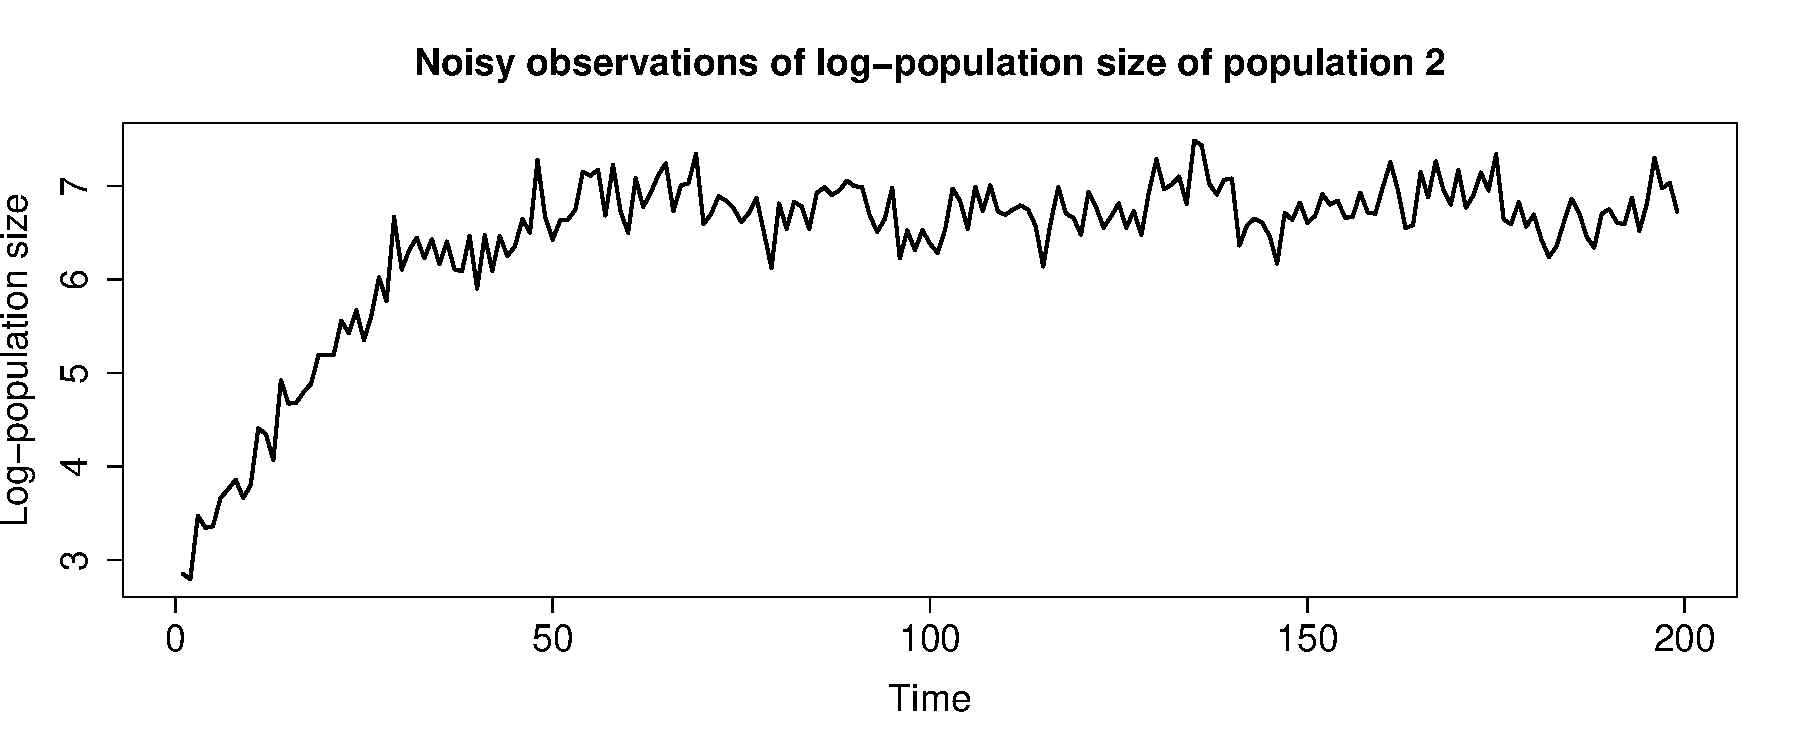
\includegraphics[width=250px]{../plots/dataset-2.pdf}
    \end{figure}
\end{frame}

\begin{frame}{The Model}
    Non-linear state space model.
    \begin{align*}
        P_t &= P_{t-1} + r_0 \left(1 - \left[\frac{\exp{(P_{t-1})}}{K}\right]^\theta\right) + e_t \\
        X_t &= P_t + u_t
    \end{align*}
    \begin{itemize}
        \item $P_t$ is log-population size. $e_t\sim N(0, Q)$ and $u_t\sim N(0,R)$ are iid.
        \item The parameter vector is $\myvec{\lambda} = (\theta, r_0, K, Q, R)$ and all parameters are assumed positive.
    \end{itemize}
\end{frame}

\begin{frame}{Discretization of model}
    \begin{itemize}
        \item Assume the state $P_t$ is bounded on an interval $[a_0,a_1]$
        \item Partition $[a,b]$ into $m$ intervals $\Omega_i=(b_{i-1},b_i)$
        \item The width of each interval is then $w=(a_1-a_0)/m$
        \item And the boundaries are $b_i=a_0+wi$
        \item Introduce discrete, integer valued state-space variables $C_t$.
        \item If $P_t\in\Omega_i$ then $C_t=i$.
        \item To link $P_t$ and $C_t$ the discrete state $i$ is represented by the midpoint $p_i=a_0+w(i-0.5)$
    \end{itemize}
\end{frame}

\begin{frame}{Discretization of model continued}
    \begin{itemize}
        \item The state dependent distribution is then given by
        \begin{equation*}
            X_t\given C_t=i\:\sim\:N(p_i, R)
        \end{equation*}
        \item And the transition probabilities as
        \begin{align*}
            P(C_t=j\given C_{t-1}=i) &= \int_{\Omega_j} n(p_t, \mu_i, Q)\,dp_t \\
                &\approx \frac{w}{2}(n(b_{j-1}, \mu_i, Q) + n(b_j, \mu_i, Q))
        \end{align*}
        where $\mu_i = p_i + r_0\left(1-\left[\frac{\exp(p_i)}{K}\right]^\theta\right)$
    \end{itemize}
\end{frame}

\begin{frame}{Computing the likelihood}
    The markov chain is not assumed stationary so instead
    \begin{equation*}
        \myvec{\phi}_1 = \frac{\myvec{1}\myvec{P}(x_1)}{\myvec{1}\myvec{P}(x_1)\myvec{1^{'}}}
    \end{equation*}
    is used as the initial distribution.
    \\
    Since all parameters $\myvec{\lambda} = (\theta, r_0, K, Q, R)$ are assumed positive they can easily be transformed to unconstrained working parameters by 
    \begin{equation*}
        \myvec{\tau}=\log\myvec{\lambda}\quad\text{and back}\quad \myvec{\lambda}=\exp{\myvec{\tau}}
    \end{equation*}
\end{frame}

\begin{frame}{Parameter estimates}
    Parameter estimates for dataset 1
    \begin{table}[htb]
        \begin{tabular}{lr|rr|r}
             & \multicolumn{1}{r}{Estimate} & \multicolumn{2}{c}{95\% Conf.Int} & Std.Dev \\\hline
            $\theta$ & 0.4615 & -0.3769 & 1.3000 & 0.4278\\$r_0$ & 0.1423 & -0.0315 & 0.3160 & 0.0886\\$K$ & 822.9574 & 631.7430 & 1014.1718 & 97.5584\\$Q$ & 0.0090 & 0.0037 & 0.0144 & 0.0027\\$R$ & 0.0407 & 0.0304 & 0.0510 & 0.0053 \\
        \end{tabular}
    \end{table}
    Is it sensible to assume that $\theta$ and/or $r_0$ is 0?\\
\end{frame}

\begin{frame}{Is it sensible?}
    The model is then
    \begin{align*}
        P_t &= P_{t-1} + e_t \\
        X_t &= P_t + u_t
    \end{align*}
    which gives
    \begin{align*}
        X_t &= X_{t-1} + P_t - P_{t-1} + u_t - u_{t-1} \\
        &= X_{t-1} + e_t + u_t - u_{t-1}
    \end{align*}
    and since $\epsilon_t = e_t + u_t - u_{t-1}\sim N(0, 2R+Q)$ is just white noise, we get the random walk process
    \begin{align*}
        X_t = X_{t-1} + \epsilon_t
    \end{align*}
\end{frame}

\begin{frame}{Is it sensible?}
    \begin{figure}
    \includegraphics[width=250px]{../plots/dataset-1.pdf}
    \end{figure}
    \begin{figure}
    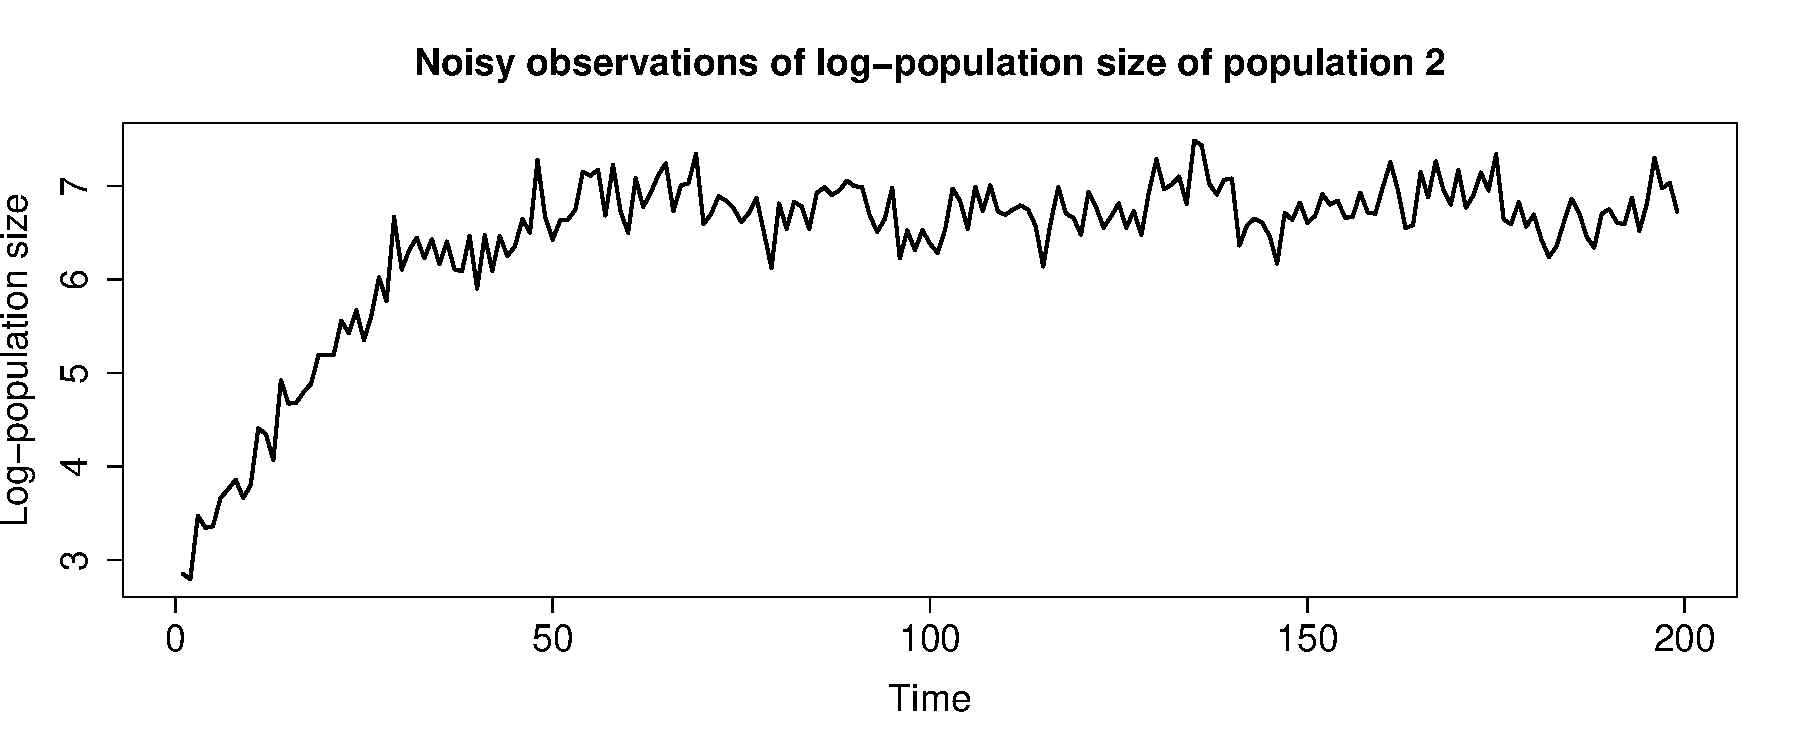
\includegraphics[width=250px]{../plots/dataset-2.pdf}
    \end{figure}
\end{frame}

\begin{frame}{Correlation of estimates}
    The model
    \begin{align*}
        P_t &= P_{t-1} + r_0 \left(1 - \left[\frac{\exp{(P_{t-1})}}{K}\right]^\theta\right) + e_t \\
        X_t &= P_t + u_t
    \end{align*}
    Correlation of parameter estimates
    \begin{align*}
        \Corr{\widehat{\theta}, \widehat{r_0}} = -0.954,\:
        \Corr{\widehat{Q}, \widehat{R}} = -0.315, \:
        \Corr{\widehat{\theta}, \widehat{Q}} = 0.247
    \end{align*}
\end{frame}

\begin{frame}{Local decoding}
    \begin{figure}
        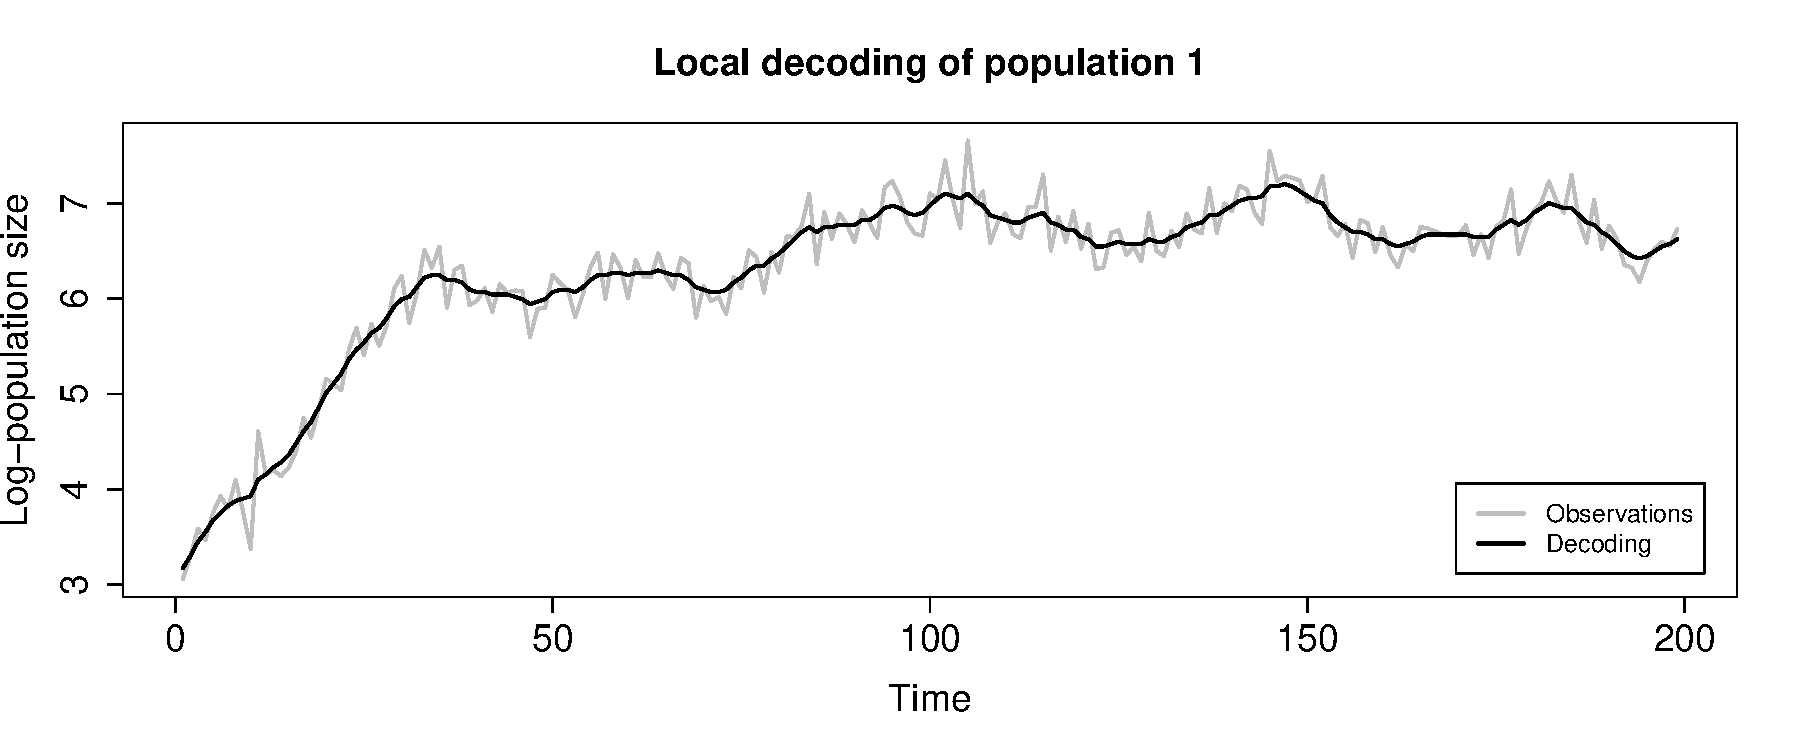
\includegraphics[width=240px]{../plots/cont-dataset-1-param-1-decoding.pdf}\\
        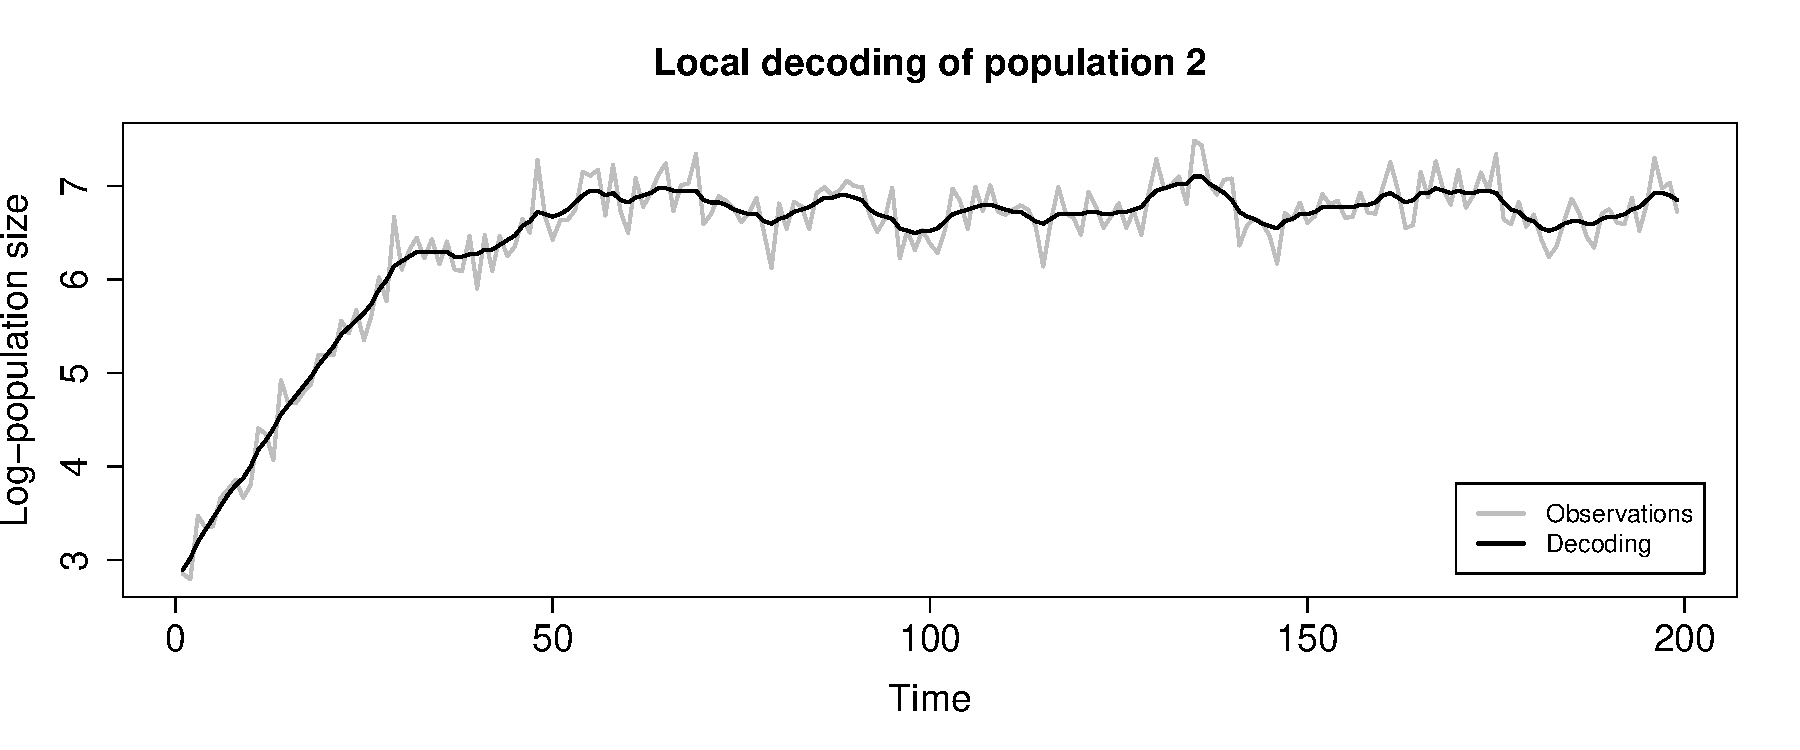
\includegraphics[width=240px]{../plots/cont-dataset-2-param-1-decoding.pdf}
    \end{figure}
\end{frame}


\begin{frame}{Questions}
    Time for some questions...
\end{frame}


\end{document}
